% !TeX spellcheck = en_US
% !TeX encoding = utf8
% !TeX program = xelatex
% !BIB program = bibtex

% \documentclass{beamer}
\documentclass[notes]{beamer}
% \documentclass[draft]{beamer}	
% \usetheme{Singapore}
% \usetheme{Hannover}
% \usepackage{pgfpages}
%\setbeameroption{hide notes} % Only slides
%\setbeameroption{show only notes} % Only notes
% \setbeameroption{show notes on second screen=right} % Both

\usepackage[british]{babel}
\usepackage{graphicx,hyperref,url}
% \usepackage{ru}
\usepackage{mmstyles}
% \usepackage{hanging}
\usepackage{listings}
% \usefonttheme[onlymath]{serif}
\usepackage{fontspec,xunicode}
% \setmainfont{Tahoma}
\usepackage[slantfont,boldfont]{xeCJK}
\pgfdeclareimage[width=\paperwidth,height=\paperheight]{bg}{background}
\setbeamertemplate{background}{\pgfuseimage{bg}}

\usepackage[backend=biber]{biblatex}
% \usepackage{biblatex}
\bibliography{./ref.bib}
\addbibresource{ref.bib}

\usepackage{indentfirst}
\usepackage{longtable}
\usepackage{float}
% \usepackage{picins}
\usepackage{rotating}
\usepackage{subfigure}
\usepackage{tabu}
\usepackage{amsmath}
\usepackage{amssymb}
\usepackage{setspace}
\usepackage{amsfonts}
\usepackage{appendix}
\usepackage{listings}
\usepackage{xcolor}
\usepackage{geometry}

\setmainfont{Times New Roman}%缺省英文字体.serif是有衬线字体sans serif无衬线字体
\setCJKmainfont[ItalicFont={Adobe Kaiti Std}, BoldFont={Adobe Heiti Std}]{STSong}%衬线字体 缺省中文字体为
\setCJKsansfont{STSong}
\setCJKmonofont{STFangsong}%中文等宽字体
%%-----------------------xeCJK下设置中文字体------------------------------%
\setCJKfamilyfont{song}{SimSun}                             %宋体 song
\newcommand{\song}{\CJKfamily{song}}
\setCJKfamilyfont{fs}{FangSong_GB2312}                      %仿宋2312 fs
\newcommand{\fs}{\CJKfamily{fs}}
\setCJKfamilyfont{yh}{Microsoft YaHei}                    %微软雅黑 yh
\newcommand{\yh}{\CJKfamily{yh}}
\setCJKfamilyfont{hei}{SimHei}                              %黑体  hei
\newcommand{\hei}{\CJKfamily{hei}}
\setCJKfamilyfont{hwxh}{STXihei}                                %华文细黑  hwxh
\newcommand{\hwxh}{\CJKfamily{hwxh}}
\setCJKfamilyfont{asong}{Adobe Song Std}                        %Adobe 宋体  asong
\newcommand{\asong}{\CJKfamily{asong}}
\setCJKfamilyfont{ahei}{Adobe Heiti Std}                            %Adobe 黑体  ahei
\newcommand{\ahei}{\CJKfamily{ahei}}
\setCJKfamilyfont{akai}{Adobe Kaiti Std}                            %Adobe 楷体  akai
\newcommand{\akai}{\CJKfamily{akai}}

\newcommand{\verylarge}{\fontsize{60pt}{\baselineskip}\selectfont}  
\newcommand{\chuhao}{\fontsize{44.9pt}{\baselineskip}\selectfont}  
\newcommand{\xiaochu}{\fontsize{38.5pt}{\baselineskip}\selectfont}  
\newcommand{\yihao}{\fontsize{27.8pt}{\baselineskip}\selectfont}  
\newcommand{\xiaoyi}{\fontsize{25.7pt}{\baselineskip}\selectfont}  
\newcommand{\erhao}{\fontsize{23.5pt}{\baselineskip}\selectfont}  
\newcommand{\xiaoerhao}{\fontsize{19.3pt}{\baselineskip}\selectfont} 
\newcommand{\sihao}{\fontsize{14pt}{\baselineskip}\selectfont}      % 字号设置  
\newcommand{\xiaosihao}{\fontsize{12pt}{\baselineskip}\selectfont}  % 字号设置  
\newcommand{\wuhao}{\fontsize{10.5pt}{\baselineskip}\selectfont}    % 字号设置  
\newcommand{\xiaowuhao}{\fontsize{9pt}{\baselineskip}\selectfont}   % 字号设置  
\newcommand{\liuhao}{\fontsize{7.875pt}{\baselineskip}\selectfont}  % 字号设置  
\newcommand{\qihao}{\fontsize{5.25pt}{\baselineskip}\selectfont}    % 字号设置 

\graphicspath{{./fig/}}

% \setbeamertemplate{footnote}{%
%   \hangpara{2em}{1}%
%   \makebox[2em][l]{\insertfootnotemark}\footnotesize\insertfootnotetext\par%
% }

\definecolor{cred}{rgb}{0.6,0,0}
\definecolor{cgreen}{rgb}{0.25,0.5,0.35}
\definecolor{cpurple}{rgb}{0.5,0,0.35}
\definecolor{cdocblue}{rgb}{0.25,0.35,0.75}
\definecolor{cdark}{rgb}{0.95,1.0,1.0}
\lstset{
	language=R,
	numbers=left,
	numberstyle=\tiny\color{black},
	keywordstyle=\color{cpurple}\consolas,
	commentstyle=\color{cgreen}\consolas,
	stringstyle=\color{cred}\consolas,
	frame=single,
	escapeinside=``,
	xleftmargin=1em,
	xrightmargin=1em, 
	backgroundcolor=\color{cdark},
	aboveskip=1em,
	breaklines=true,
	tabsize=3
} 

\makeatletter
\long\def\beamer@author[#1]#2{%
  \def\insertauthor{\def\inst{\beamer@insttitle}\def\and{\beamer@andtitle}%
  \begin{tabular}{rl}#2\end{tabular}}%
  \def\beamer@shortauthor{#1}%
  \ifbeamer@autopdfinfo%
    \def\beamer@andstripped{}%
    \beamer@stripands#1 \and\relax
    {\let\inst=\@gobble\let\thanks=\@gobble\def\and{: }\hypersetup{pdfauthor={\beamer@andstripped}}}
  \fi%
}
\makeatother

% \setbeamersize{text margin left=60mm} 
\setbeamertemplate{frametitle}[default][right]

% The title of the presentation:
%  - first a short version which is visible at the bottom of each slide;
%  - second the full title shown on the title slide;
\title[毕设开题]{毕业论文开题答辩}

% Optional: a subtitle to be dispalyed on the title slide
\subtitle{深度行人再识别学习}

% The author(s) of the presentation:
%  - again first a short version to be displayed at the bottom;
%  - next the full list of authors, which may include contact information;
\author[xinglu]{ 
	姓名学号: & 王兴路 3140102282 \\
指导老师: & 李英明 \\
年级专业: & 2014级信息工程
}
% The institute:
%  - to start the name of the university as displayed on the top of each slide
%    this can be adjusted such that you can also create a Dutch version
%  - next the institute information as displayed on the title slide

\institute[信工1403]{}

% Add a date and possibly the name of the event to the slides
%  - again first a short version to be shown at the bottom of each slide
%  - second the full date and event name for the title slide
\date[\today]{}

\begin{document}

\AtBeginSection[]
{
	\begin{frame}
		\frametitle{大纲}
		\tableofcontents[currentsection]
	\end{frame}
}

% \AtBeginSubsection[2-]
% {
%    \begin{frame}
%        \frametitle{Outline}
%        \tableofcontents[currentsection]
%    \end{frame}
% }

\begin{frame}
	\titlepage
\end{frame}

\section{背景介绍}
\begin{frame}{背景}
	

\end{frame}

% \begin{frame}{test}
% 	\begin{columns}

% 		\column{0.49\textwidth}
% 		This is a text in first column.
% 		$$E=mc^2$$

% 		\column{0.49\textwidth}
% 		This text will be in the second column
% 		and on a second tought this is a nice looking
% 		layout in some cases.
% 	\end{columns}
% \end{frame}
\begin{frame}
	{行人再识别定义}
	行人再识别(Person Re-identification,简称 ReID) , 也称行人重识别
	是利用计算机视觉技术,在图像或者视频集合(gallery)中找到与询问图片(query)相
	似行人的任务。
	

	\begin{figure}
		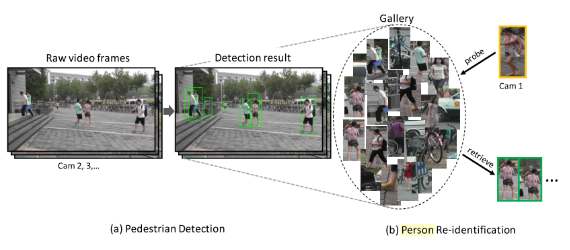
\includegraphics[width=0.7\linewidth]{2018-03-07-19-55-19.png}
	\end{figure}
\end{frame}

\begin{frame}
	{背景介绍}
	\begin{itemize}
		\item 行人再识别在智能视频监控、智能安防邻域广泛应用
		\item 单个摄像头视野有限,如何\textit{跨摄像头}跟踪行人
		\item 摄像头采集了\emph{海量}数据,如何利用、如何大规模检索
	\end{itemize}
	\begin{figure}
		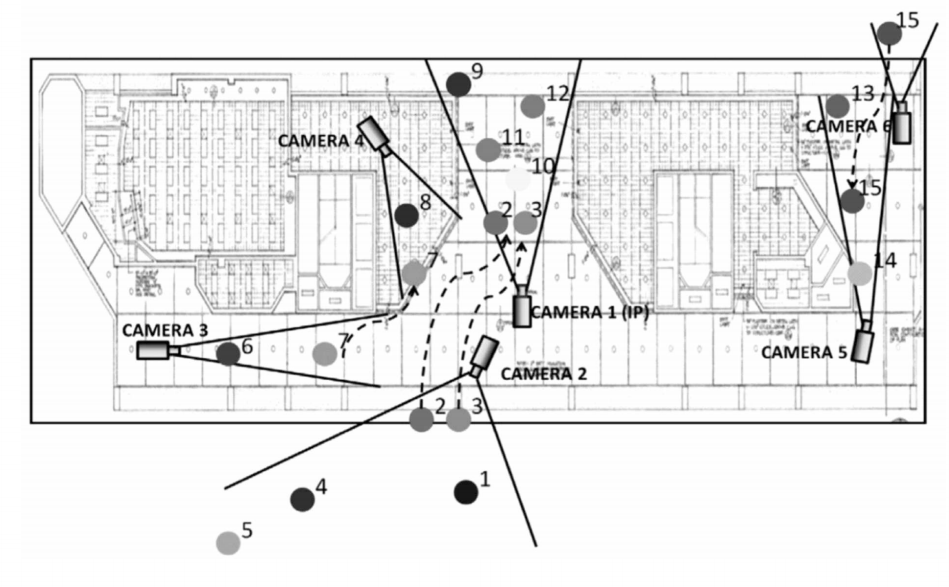
\includegraphics[width=0.7\linewidth]{2018-03-07-19-33-13.png}
	\end{figure}
\end{frame}




\section{研究意义和目的}
\begin{frame}
	{存在的挑战}

	\begin{figure}
		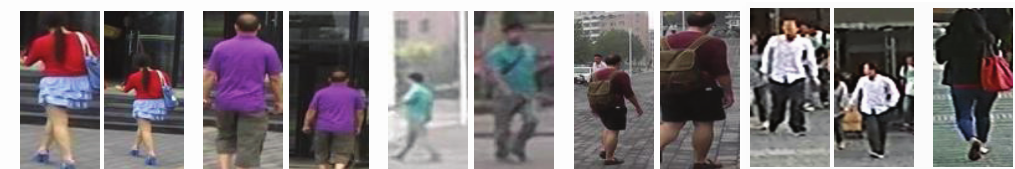
\includegraphics[width=0.7\linewidth]{2018-03-07-20-16-25.png}
	\end{figure}
	the learning of comprehensive features of pedestrians for fine-grained tasks remains an open problem.
	\note{
		 Desired features for open-set FR are expected to satisfy
		the criterion that the maximal intra-class distance is smaller than the minimal inter-class distance under a certain metric space. This
		 由于行人的非刚性运动、检测器的误差、摄像头的
		视角变化,同一行人的不同图片往往存在严重的空间失配(Spatial Misalignment);行
		人没有可靠的生物特征,只能从属性、语义层面的特征加以区分;未标定的摄像机参
		数、巨大的时空跨度,这些都进一步增加了再识别的难度;同时现有的数据集规模相
		对较小,不存在 ImageNet 或者 MegaFace 这样的大规模、可以泛化迁移(Transfer)到
		任意子领域(domain)的数据集。这导致数据集间存在较大偏差(domain bias/domain
		shift),从一个数据集到另一个数据集,
		模型的性能通常都会下降。
	}
\end{frame}

\section{主要研究内容}

\section{技术路线与设计方案}

\section{进度安排与预期目标}
\begin{frame}
	{进度安排}
	毕业设计(论文)各阶段工作内容:(此处较简较泛泛,应参照同学与指导老师交流讨论定的详细进度安排缩写)
	2012年11月19日~2013年3月8日:专题研究
	2011年11月19日~2013年3月8日:开题,完成外文文献翻译、文献综述、开题报告并开题答辩
	2013年3月29日~4月28日:进一步学习相关技术,硬件电路设计,进行软件部分编程与调试
	2013年4月29日~5月29日:软硬件调试,功能测试,性能优化
	2013年5月30日~6月上旬:撰写毕业论文,答辩 \cite{markowitz1952portfolio}

\end{frame}





\begin{frame}[t, allowframebreaks]
\frametitle{References}


\printbibliography
\end{frame}

\begin{frame}
	\chuhao Thank you! %\fontspec{LHANDW.TTF}
\end{frame}


\end{document}
